\begin{figure}[!htbp]
	\begin{subfigure}{\linewidth}
		\centering
        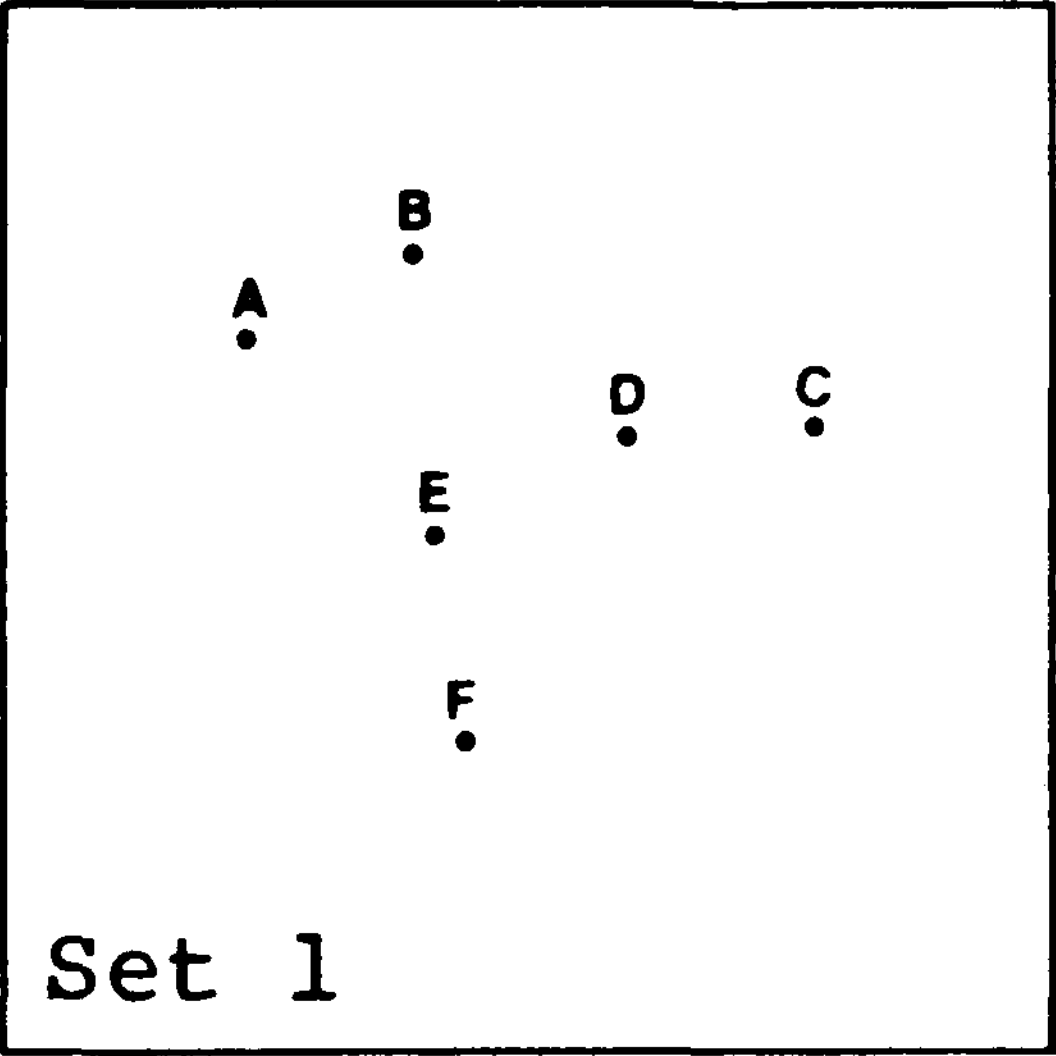
\includegraphics[width=.48\textwidth]{figures/registration/convex/set1.png}
        \raisebox{1px}{
			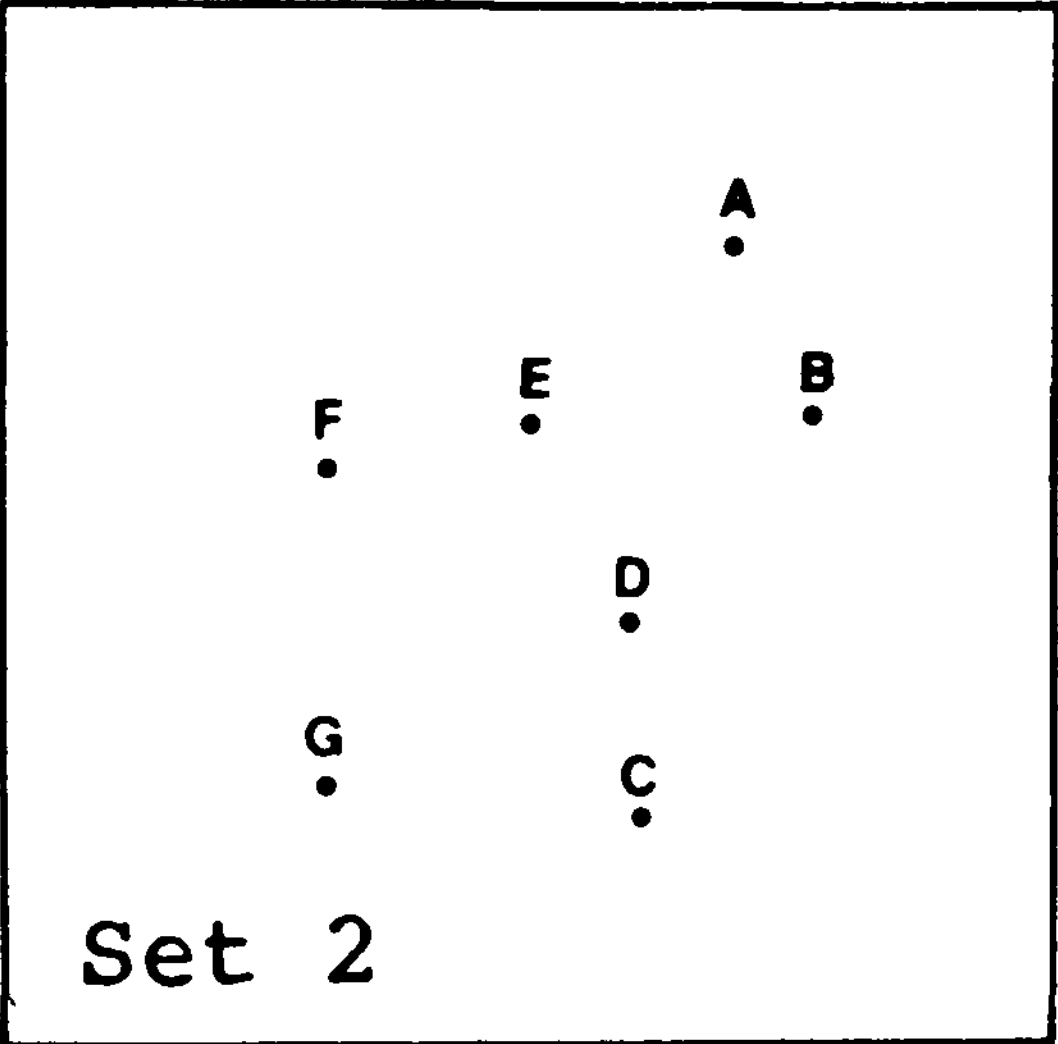
\includegraphics[width=.48\textwidth]{figures/registration/convex/set2.png}
		}
		\caption{Two sets of points. Set 2 is 90 degrees rotated and has extra point \(G\).} \label{fig:twosetsofpoints}
	\end{subfigure}
	\vskip\baselineskip
	\begin{subfigure}{\linewidth}
		\centering
		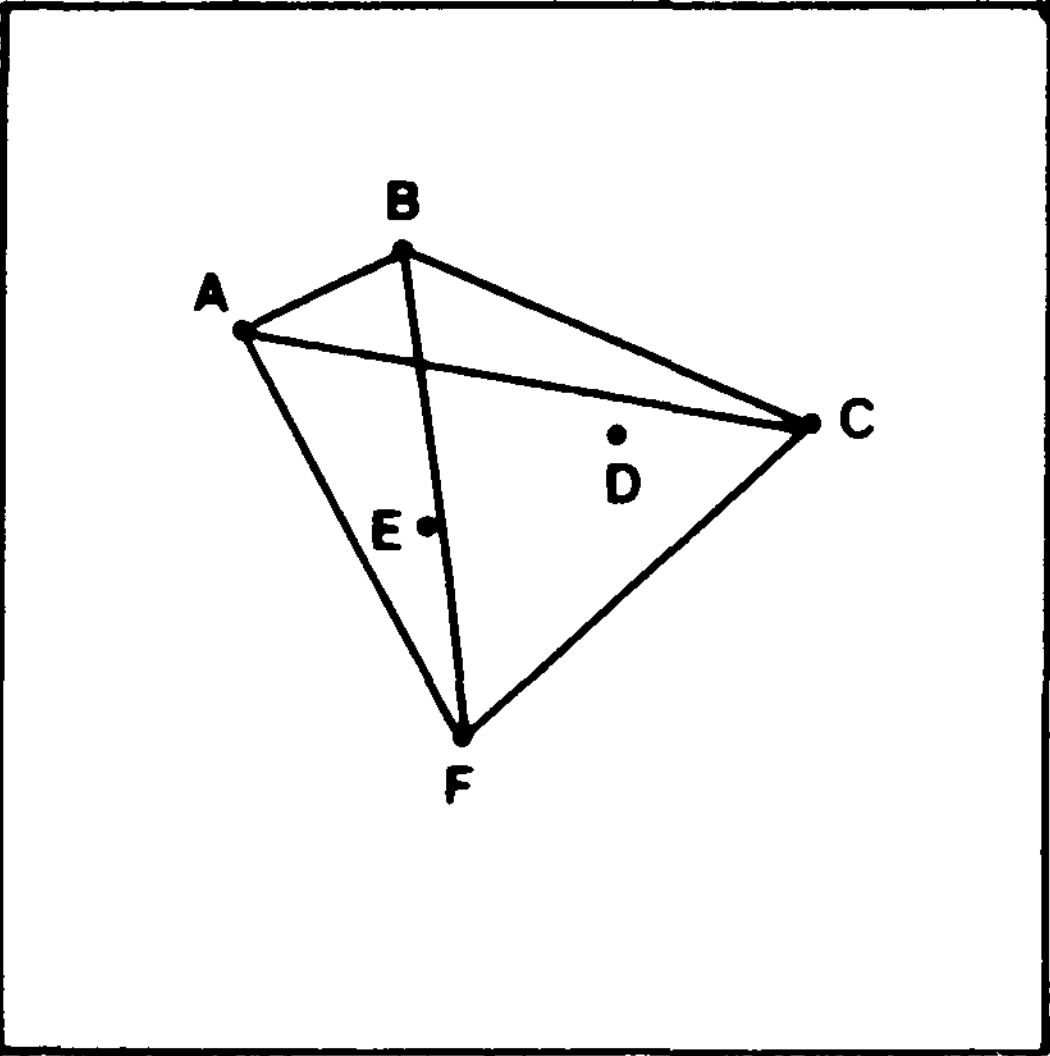
\includegraphics[width=.48\textwidth]{figures/registration/convex/complete_graph_set1.png}
		\raisebox{0.5px}{
			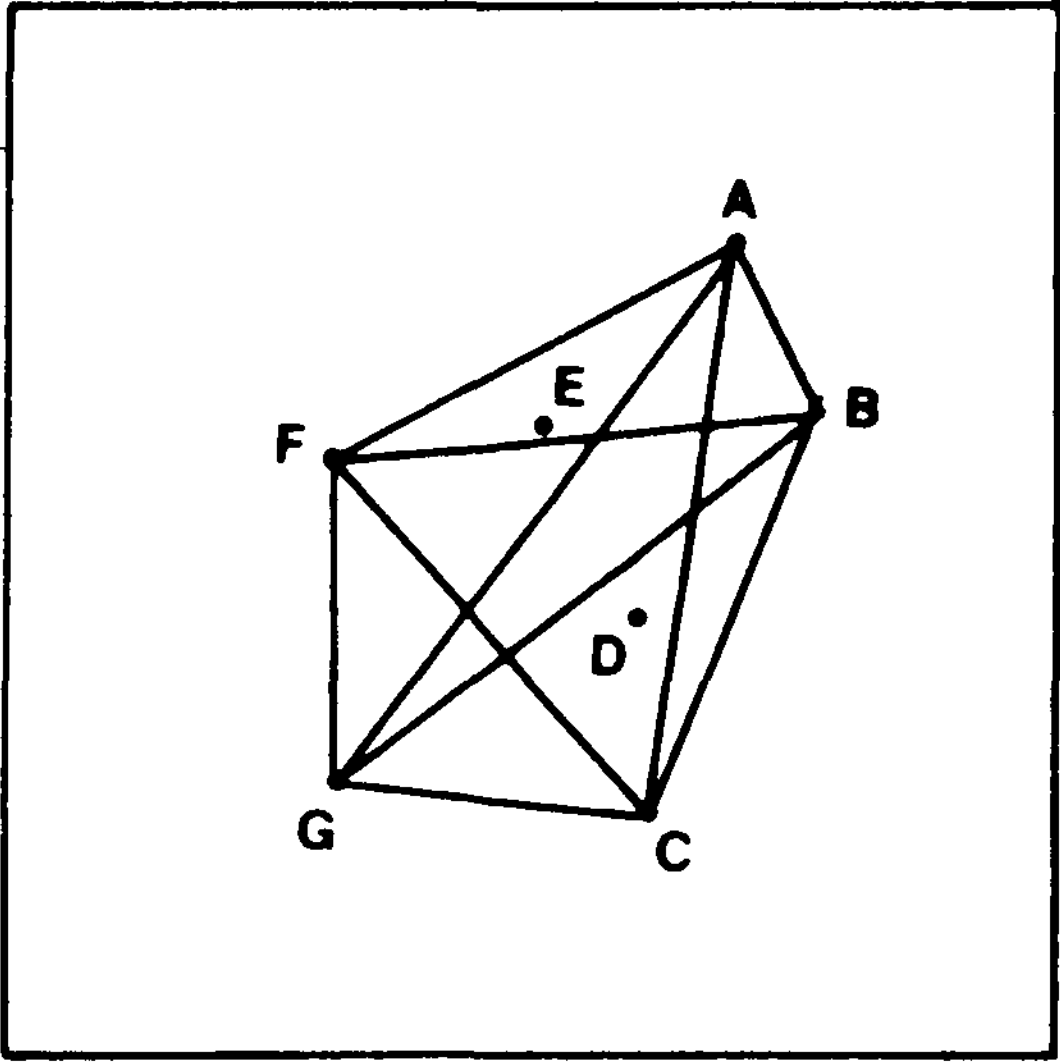
\includegraphics[width=.48\textwidth]{figures/registration/convex/complete_graph_set2.png}
		}
		\caption{Convex hull complete graph edges of two sets, used by the point matching using convex hull edges algorithm.} \label{fig:twoconvexcomplete}
	\end{subfigure}
	\caption{Point matching using convex hull edges \cite{Goshtasby1985}.}
	\label{fig:convexhulledges}
\end{figure}
